\chapter{Implementazione} %\label{1cap:spinta_laterale}
% [titolo ridotto se non ci dovesse stare] {titolo completo}
%

\begin{citazione}
Nell'ambito del presente capitolo verranno trattate le scelte effettuate per l'implementazione degli algoritmi facenti parte della \emph{pipeline} di compressione. Verrà posta particolare attenzione ai dettagli implementativi della \emph{sBWT} in quanto risulta essere l'algoritmo più pesante in termini di spazio occupato e di tempo impiegato. Verrà, successivamente, fornita una descrizione delle strategie impiegate per l'implementazione della \emph{bMTF} e della \emph{RLE}. Il capitolo si conclude con la descrizione della scelta dell'algoritmo di \emph{Variable Length Prefix Code} da utilizzare. 
\end{citazione}
\newpage

\section{Panoramica sullo sviluppo dell'algoritmo} 
La scelta del linguaggio di programmazione da utilizzare per l'implementazione dell'algoritmo di compressione sicuro è ricaduta su \emph{Python}. Tale scelta è stata guidata dalla ricerca di un linguaggio semplice e flessibile che consentisse di implementare in modo agevole e veloce gli algoritmi descritti soffermandosi sui dettagli rilevanti. Il codice sorgente dell'algoritmo sviluppato è reperibile al seguente link: https://github.com/vincenzo-emanuele/Progetto-Compressione-Dati. Come mostrato nella figura \ref{fig:project} il progetto è stato suddiviso in 4 \emph{packages}: \emph{sbwt, bmtf, pc e rle}, ognuno dei quali contiene il codice sorgente del corrispondente algoritmo della \emph{pipeline}. L'implementazione delle \emph{pipeline} di compressione e di decompressione è demandato a due file che fungono da tester dei due processi, denominati \emph{compressione.py} e \emph{decompressione.py}. La \emph{pipeline} complessiva è implementata dal file \emph{tester.py} che orchestra l'esecuzione invocando il modulo di compressione e quello di decompressione. La cartella \emph{TestFiles} contiene i file input utilizzati per testare l'algoritmo con i relativi file output prodotti dal processo di compressione.
\begin{figure}[h]
    \centering
    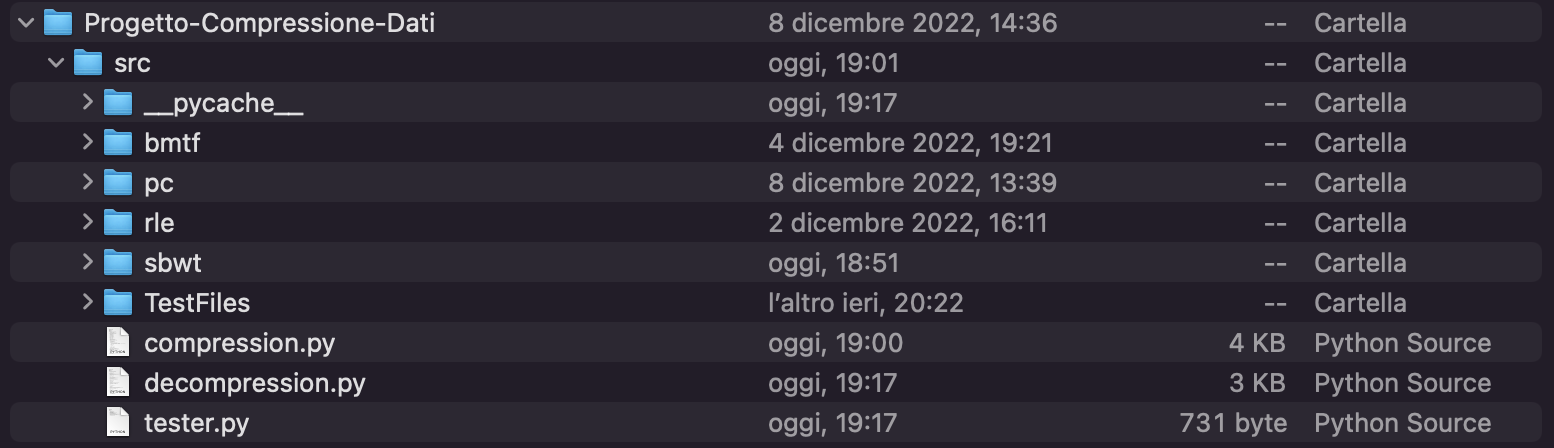
\includegraphics[width=1\textwidth]{Progetto Compressione Dati/capitoli/images/project.png}
\caption{Struttura del progetto}
    \label{fig:project}
\end{figure} \\
\section{Implementazione della sBWT} 
La prima importante questione da affrontare in fase di implementazione della \emph{sBWT} riguarda la realizzazione del layer di sicurezza che si concretizza nell'utilizzo di una chiave segreta per computare un ordinamento lessicografico segreto da utilizzare in fase di disposizione delle righe della matrice.
Risulta, inoltre, necessario affrontare la questione relativa alle prestazioni dell'algoritmo. Implementare la \emph{sBWT} seguendo gli step dell'algoritmo, infatti, non risulta praticabile in quanto la costruzione della matrice porterebbe ad un'esplosione della complessità in termini di tempo e di spazio. Per avere un'idea sulla complessità totale, basti pensare al fatto che la matrice da costruire contiene un numero di elementi pari al quadrato del numero di caratteri della stringa da comprimere; ciò significa che un file di appena 1MB porterebbe alla costruzione di una matrice di 1.099.511.627.776 elementi, occupando oltre 1TB di memoria. Per evitare tali situazioni è possibile applicare diverse ottimizzazioni che poggiano le proprie fondamenta sul fatto di lavorare sulla matrice senza costruirla esplicitamente, facendo uso di strutture ausiliarie costruite \emph{ad-hoc}. I paragrafi successivi descrivono nel dettaglio l'implementazione del layer di sicurezza e le ottimizzazioni attuate.
\subsection{Implementazione del layer di sicurezza}
Nell'ambito del presente lavoro, la realizzazione del layer di sicurezza della \emph{sBWT} è un'implementazione del lavoro svolto dagli autori di \cite{zeng2018secure}. Una descrizione ad alto livello del funzionamento della \emph{sBWT} è stata fornita nel paragrafo \ref{section:sbwt} ed è stata implementata dagli \emph{script} del \emph{package sbwt}. Lo scopo di questo layer di sicurezza è quello di ottenere una permutazione dell'alfabeto su cui è definita la stringa input da comprimere. Nello specifico, mediante la libreria \emph{random} di \emph{Python} viene generato un numero casuale $r$ da 0 a 9999999 che viene salvato su un file denominato \emph{rfile.txt}. A tale $r$ viene accodata la chiave segreta $K$ fornita in input eventualmente dall'utente dell'algoritmo. La chiave risultante $Key=r+K$ viene utilizzata come seed per il generatore di numeri casuali fornito dalla libreria \emph{random} di \emph{Python} mediante il quale vengono generati valori attribuiti a ciascun carattere dell'alfabeto da permutare. In fase di disposizione delle righe della matrice, l'algoritmo di ordinamento farà uso di tale associazione \emph{simbolo dell'alfabeto-numero casuale} creando, così, una permutazione dell'alfabeto input. Tale algoritmo risulta invertibile a patto di salvare il numero casuale $r$ e di conoscere la chiave $K$; infatti, l'utilizzo dello stesso seed $Key=r+K$ fa sì che i numeri casuali ottenuti dal generatore siano esattamente gli stessi, garantendo, in questo modo, l'ottenimento della permutazione dell'alfabeto utilizzata in fase di compressione.
\subsection{Suffix Array}
Al fine di evitare la costruzione esplicita della matrice della \emph{BWT} sono stati utilizzati i \textbf{suffix array}, una struttura dati ben nota nell'ambito degli algoritmi. Formalmente, data una stringa $S$, il \emph{suffix array} $A$ di $S$ è un array di interi contenente le posizioni iniziali dei suffissi di $S$ in ordine lessicografico. Ad esempio, data la stringa $S=banana\$$ (\$ è il carattere speciale di \emph{EOF}), si indicizza la stringa come illustrato nella figura \ref{fig:sa1}.
\begin{figure}[h]
    \centering
    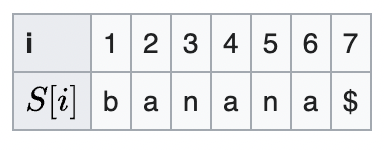
\includegraphics[scale=0.80]{Progetto Compressione Dati/capitoli/images/sa1.png}
\caption{Fonte: https://en.wikipedia.org/wiki/Suffix\_array}
    \label{fig:sa1}
\end{figure}\\
Successivamente si considerano tutti i suffissi: \{\emph{banana\$, anana\$, nana\$, ana\$, na\$, a\$, \$}\} e li si dispone in ordine lessicografico come illustrato nelle figure \ref{fig:sa2} e \ref{fig:sa3}.
\begin{figure}[h]
    \centering
    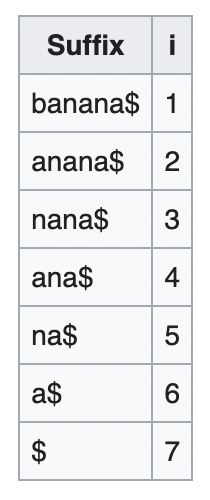
\includegraphics[scale=0.60]{Progetto Compressione Dati/capitoli/images/sa2.png}
\caption{Fonte: https://en.wikipedia.org/wiki/Suffix\_array}
    \label{fig:sa2}
\end{figure}
\begin{figure}[h]
    \centering
    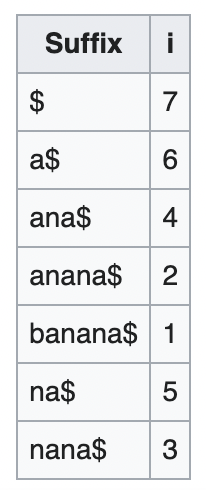
\includegraphics[scale=0.60]{Progetto Compressione Dati/capitoli/images/sa3.png}
\caption{Fonte: https://en.wikipedia.org/wiki/Suffix\_array}
    \label{fig:sa3}
\end{figure}\\
Il \emph{suffix array} risultante sarà $S=\{7, 6, 4, 2, 1, 5, 3\}$. Chiarito il funzionamento della struttura dati in questione, risulta utile descrivere il modo in cui la \emph{sBWT} la utilizza. La matrice $M$ utilizzata dalla \emph{sBWT} contiene, su ogni riga, tutti i suffissi di $S$ ordinati in ordine lessicografico. L'algoritmo computa, in primo luogo, il \emph{suffix array} $A$ relativo a $S$. Dal momento che tale \emph{array} contiene gli indici di tutti i suffissi di $S$ ordinati in ordine lessicografico, vi sarà una corrispondenza biunivoca tra le righe di $M$ e i suffissi "puntati" dagli indici di $A$. In particolare, la \emph{i-esima} riga di $M$ inizierà con il suffisso "puntato" dall'\emph{i-esimo} elemento di $A$. Risulta, dunque, immediato risalire all'ultimo carattere dell'\emph{i-esima} riga di $M$ in quanto sarà proprio l'\emph{i-1-esimo} carattere di $L$. \\ L'ottimizzazione appena descritta riduce la complessità spaziale della \emph{sBWT} da \emph{quadratica} a \emph{lineare}. La complessità temporale, invece, dipende dall'implementazione scelta per la costruzione dei \emph{suffix array}; nell'implementazione proposta dal presente lavoro è stata utilizzata un'implementazione avente complessità $\mathcal{O}(n\log^2{}n)$. Dal momento che la \emph{sBWT}, una volta aver ottenuto il \emph{suffix array}, computa il suo output in tempo $\mathcal{O}(n)$, l'algoritmo complessivo avrà complessità totale $\mathcal{O}(n\log^2{}n)$. La costruzione dei \emph{suffix array} è implementata dalla classe \emph{suffix.py} situata nel package \emph{sbwt}.
\subsection{Variante a blocchi e parallelizzazione}
Al fine di ridurre il tempo richiesto dalla compressione, la \emph{sBWT} viene eseguita su blocchi dell'input di taglia fissata. La dimensione da usare per il blocco è stata scelta in maniera "empirica"; intuitivamente un blocco di dimensione troppo piccola rende meno efficace il raggruppamento dei caratteri effettuato dalla \emph{sBWT} mentre un blocco di dimensione troppo grande rende il \emph{processing} di ciascuno di questi troppo oneroso. Un buon compromesso si ottiene lavorando con blocchi aventi dimensione \emph{300 kB}. Grazie al supporto di \emph{Python} al \emph{multiprocessing} (fornito dalla libreria \emph{multiprocessing}), il \emph{processing} dei blocchi avviene in parallelo, apportando un ulteriore miglioramento al tempo di esecuzione dell'algoritmo.
\subsection{Calcolo dell'inversa}
Il calcolo dell'inversa della trasformata è implementato evitando la costruzione esplicita della matrice al fine di scongiurare un'esplosione della complessità. Il paper \cite{burrows1994block} propone una strategia per il calcolo dell'inversa della \emph{BWT} che evita la costruzione della matrice. L'algoritmo prende in input il risultato $L$ della \emph{sBWT}, l'ordinamento lessicografico $O$ utilizzato in fase di compressione e restituisce la stringa non compressa $S$ facendo uso di strutture ausiliarie denominate $C$ e $P$:
\begin{itemize}
    \item $C$ è un dizionario costruito in modo tale che $C[ch]$ è il numero totale di istanze in $L$ dei caratteri che precedono $ch$ nell'ordinamento definito sull'alfabeto;
    \item $P$ è una lista costruita in modo tale che $P[i]$ è il numero di istanze del carattere $L[i]$ nel prefisso $L[0,\dots,i-1]$ di $L$;
\end{itemize}
\begin{figure}[h]
    \centering
    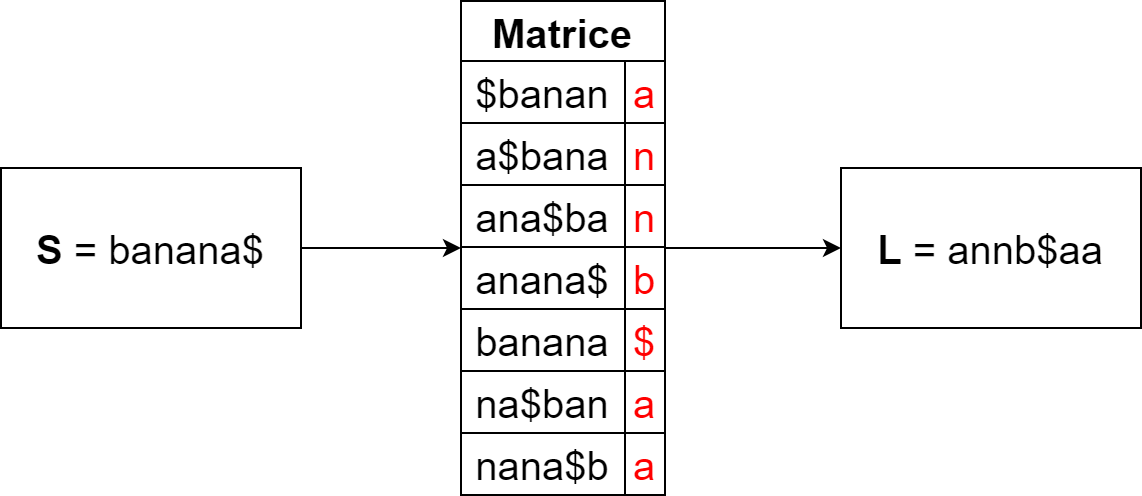
\includegraphics[width=1\textwidth]{Progetto Compressione Dati/capitoli/images/ibwt_ex.png}
\caption{Struttura del progetto}
    \label{fig:ibwt_ex}
\end{figure} \\
Grazie a tali strutture, l'algoritmo riesce ad ottenere $S$. Le modalità mediante le quali tale stringa viene costruita si basano sul fatto che non sia necessario costruire esplicitamente una matrice per sfruttarne le proprietà. Dal momento che il funzionamento dell'algoritmo non risulta essere del tutto intuitivo, la sua trattazione verrà affrontata utilizzando come supporto un esempio pratico. Come illustrato nella figura \ref{fig:ibwt_ex} l'output restituito dalla \emph{BWT} sarà l'ultima colonna della matrice ordinata degli shift ciclici di $S$. Dal momento che il carattere di \emph{EOF} è il più piccolo secondo l'ordinamento lessicografico, la prima riga sarà sempre lo shift ciclico che come primo carattere ha l'\emph{EOF} seguito da $S$ (nel caso dell'esempio la riga $0$ della matrice è \emph{\$banana}). Ciò implica che l'ultimo carattere del testo da ricostruire (escludendo l'EOF) è il primo carattere di $L$ ($L[i]$, con $i=0$), in questo caso $a$. Dal momento che per motivi di praticità l'output verrà ricostruito al contrario, il prossimo carattere da individuare è il predecessore di $a$ in $S$. Dato che si dispone solo della stringa $L$, è necessario individuare la riga che termina con il carattere $ch$ cercato in quanto corrisponderà esattamente all'indice di $L$ contenente $ch$; tale riga conterrà i caratteri della riga appena individuata \emph{shiftati} a destra di un carattere, dunque, comincerà con $a$. Sfruttando l'ordinamento della matrice è possibile accedere agevolmente alle righe che cominciano per $a$; a tale scopo risulta utile utilizzare la struttura $C$ in quanto $C[a]$ contiene il numero di occorrenze dei caratteri precedenti ad $a$ nell'ordinamento lessicografico presenti in $L$ (in questo caso $C[a]=1$). La riga $1$ di $M$ inizierà sicuramente per $a$, tuttavia la matrice potrebbe contenere più righe che cominciano con $a$, per cui è necessario stabilire quale di queste contenga come ultimo carattere il predecessore di $a$ cercato. Per fare ciò l'algoritmo si serve della struttura $P$ in quanto $P[i]$ indica quante volte il carattere $L[i]$ (in questo caso $a$) appare all'interno del prefisso $L[0,\dots,i-1]$. Il valore $P[i]$ fungerà da \emph{offset} indicando, tra tutte le righe che cominciano con $a$, quella desiderata. A questo punto, l'algoritmo pone $i=C[L[i]]+P[i]$ e ripete questi passi complessivamente $n$ volte (dove $n$ è la lunghezza di $L$). Ulteriori dettagli sul funzionamento e sulla correttezza di tale algoritmo sono reperibili in \cite{burrows1994block}. 
\section{Implementazione della bMTF}
Il layer di sicurezza implementato nella \emph{bMTF} consiste, in primo luogo, nel suddividere l'input in blocchi di dimensione $L$ per poi, successivamente, eseguire il classico algoritmo di \emph{MTF} descritto nel paragrafo \ref{section:mtf}. Il vantaggio di tale operazione risiede nel fatto che cambiare l'alfabeto periodicamente rende inefficaci attacchi di tipo statistico che poggiano le loro fondamenta sul fatto che uno stesso carattere ripetuto più volte nel testo cifrato corrisponda allo stesso carattere nel testo in chiaro. In altri termini, il cifrario a sostituzione monoalfabetica implementato dalla \emph{sBWT} viene, in questo modo, trasformato in un cifrario a sostituzione polialfabetica rendendo, in questo modo, l'algoritmo aderente alla nozione di \emph{IND-CPA sicurezza}. L'algoritmo in questione è implementato dallo script \emph{bmtf.py} situato nel \emph{package bmtf}. Fa uso di un vettore di inizializzazione noto (per semplicità è \emph{hard-coded}) e di una chiave $K$ fornita eventualmente dall'utente dell'algoritmo, che risulta essere la stessa utilizzata per la \emph{sBWT}. Dopo aver suddiviso l'input in blocchi, ciascuno di dimensione $L$, calcola la permutazione dell'alfabeto da usare per codificare quello specifico blocco facendo uso di un seed $S$ ottenuto dalla concatenazione dell'hash del vettore di inizializzazione (se sta codificando il primo blocco) o dell'hash del blocco precedente (se sta codificando un blocco diverso dal primo) e della chiave $K$. Analogamente a quanto avviene per la \emph{sBWT}, la permutazione dell'alfabeto viene calcolata utilizzando $S$ come seed per il generatore di numeri casuali fornito dalla libreria \emph{random} di \emph{Python}. Un importante questione da trattare nell'ambito dell'implementazione della \emph{bMTF} riguarda la dimensione dei blocchi in cui suddividere l'input. Intuitivamente, blocchi di dimensione troppo grande portano ad un minor numero di permutazioni dell'alfabeto, mentre blocchi di dimensione troppo piccola portano ad una minore efficacia della \emph{bMTF} (in altri termini le sequenze di $0$ saranno più brevi). Il valore da assegnare a $L$ è stato scelto empiricamente ed un buon compromesso è stato raggiunto fissando $L$ a 1024 byte. 
\section{Implementazione della RLE} 
Dal punto di vista implementativo, non sono state apportate modifiche rilevanti alla \emph{RLE} rispetto alla descrizione illustrata nel paragrafo \ref{section:rle}. L'algoritmo è implementato dallo \emph{script rle.py} situato nel \emph{package rle}. 
\section{Scelta dell'algoritmo di PC} 
L'ultimo componente della \emph{pipeline} implementata è l'algoritmo di \emph{variable length Prefix Code}. La scelta dell'algoritmo di \emph{PC} da utilizzare influisce sui tempi di esecuzione e sul rapporto di compressione complessivi. Gli algoritmi di \emph{PC} impiegati nella \emph{pipeline} non sono stati sviluppati da zero ma sono state utilizzate implementazioni in \emph{Python} preesistenti. La scelta dell'algoritmo di \emph{PC} da utilizzare è stata effettuata in maniera empirica in base alle prestazioni riscontrate confrontando tempi di compressione, decompressione e rapporto di compressione; una trattazione approfondita sui risultati ottenuti dal confronto di tali algoritmi è affrontata nel paragrafo \ref{section:risultati}. Lo script \emph{pc.py} situato nel \emph{package pc} implementa gli algoritmi di \emph{PC} utilizzati consentendo, mediante l'utilizzo di un parametro input, di scegliere il compressore desiderato. 
\section{Implementazione della pipeline}
Nell'ambito dell'implementazione effettuata, gli algoritmi descritti fino a questo momento sono "orchestrati" da un modulo che funge da compressore (reperibile nel \emph{main package src} sotto il nome \emph{compression.py}) e da un modulo che funge da decompressore (reperibile nel \emph{main package src} sotto il nome \emph{decompression.py}). I due moduli vengono, a loro volta, invocati dallo script \emph{tester.py} che si occupa di simulare un \emph{workflow} completo di compressione e decompressione prendendo in input da riga di comando il nome del file da comprimere e la chiave segreta da usare durante la \emph{sBWT} e la \emph{bMTF}. Durante un'esecuzione completa dell'algoritmo di compressione vengono generati diversi file, tuttavia solo una parte di essi va conservata per poter effettuare la decompressione. In particolare i file da conservare sono i seguenti: \emph{outputDictBWT.txt}, \emph{outputPC.txt}, \emph{rfile.txt} e \emph{outputPCCodec.txt} (nel caso in cui viene utilizzato \emph{Huffman}) o \emph{outputDictLZW.txt} (nel caso in cui viene utilizzato \emph{LZW}). D'altro canto, l'algoritmo di decompressione produce un unico file denominato \emph{decompressed.txt} che risulta essere identico al file di input. Dopo l'esecuzione completa della \emph{pipeline}, lo script \emph{tester.py} si occupa di verificare che il file di input sia identico all'output della decompressione.